\documentclass[a4paper]{article}

\usepackage[T1]{fontenc}
\usepackage{textcomp}
\usepackage{amsmath, amssymb, amsthm}

\usepackage{setspace}
% figure support
\usepackage{import}
\usepackage{xifthen}
\usepackage{pdfpages}
\usepackage{transparent}
\usepackage{tabularx}

\title{Nuclear Lab Report}
\date{date}
\author{Jack Ruder and Tatum Bunnett}


\begin{document}

\doublespacing
\maketitle

\begin{figure}[htpb]
	\centering
	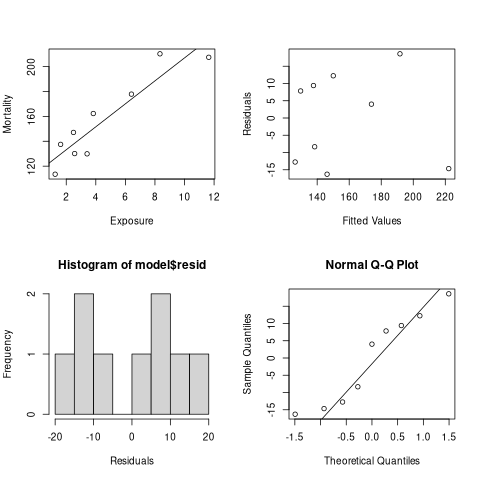
\includegraphics[width=\textwidth]{"../originalData.png"}
	\caption{Linear fit on non-transformed data}
	\label{fig:ogdat}
\end{figure}

\begin{figure}[htpb]
	\centering
	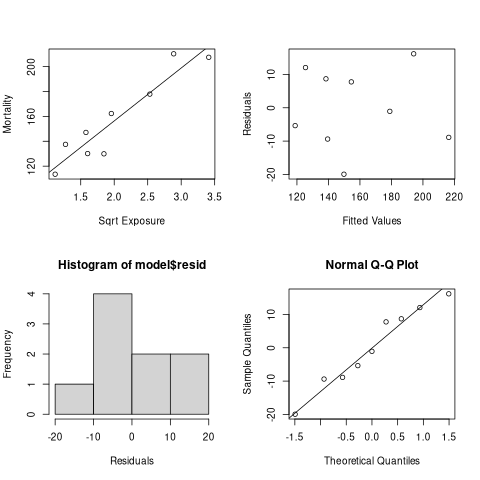
\includegraphics[width=\textwidth]{"../sqrtExposreXmortality.png"}
	\caption{Linear fit on transformed data}
	\label{fig:sqdat}
\end{figure}
\end{document}

Dear Administrators of the Hanford Nuclear Facility, 
We are concerned community members worried about radiation exposures to ourselves along with our friends and families. 
Recently, we ran statistical tests to help analyze the relationship of radiation exposure and the amount of cancer deaths in 9 different counties. 
From the results of this statistical analysis we belive that our communites are entitiled to compensation. 
Below we have listed the reasons why we belive we deserv to be compensated. 

\documentclass{article}
\usepackage{tabularx}
\begin{document}
\begin{tabularx}{0.8\textwidth} { 
  | >{\raggedright\arraybackslash}X 
  | >{\centering\arraybackslash}X 
  | >{\raggedleft\arraybackslash}X | }
 \hline
  & prediction lower & prediction upper & confidence lower & confidnece upper\\
 \hline
 low & 88.36 & 155.96 & 106.89 & 137.43 \\
 \hline
 med & 120.08 & 184.43 & 141.03 & 163.48  \\
 \hline
 high & 169.70 & 240.81 & 186.57 & 223.94 \\
\hline
\end{tabularx}
\end{document}